\documentclass[runningheads]{llncs}
\usepackage{amsmath}
\usepackage{amsfonts}
\usepackage{booktabs}
\usepackage[compress]{cite}
\usepackage{color}
\usepackage{graphicx}
\usepackage{hyperref}

\renewcommand\UrlFont{\color{blue}\rmfamily}

\begin{document}

\title{
    Ukraine Conflict Similar Tweets
}
\author{Gabriele Cerizza}
\authorrunning{G. Cerizza}

\institute{Università degli Studi di Milano\\
\email{gabriele.cerizza@studenti.unimi.it}\\
\url{https://github.com/gabrielecerizza/amd_project}}

\maketitle

\section*{Introduction}
\label{sec:introduction}

In this report we detail our findings in the study of an algorithm capable of identifying similar pairs of documents within massive datasets. The experiments illustrated hereinafter were carried out as part of a project for the Algorithms for Massive Datasets course of Università degli Studi di Milano.

In Section~\ref{sec:dataset} we illustrate the dataset and the adopted pre-processing techniques. In Section~\ref{sec:models} we briefly describe the algorithm and its implementation. We also outline the neural network model used to evaluate the performance of the algorithm. In Section~\ref{sec:experiments} we expound on the findings of our experiments. Finally, Section~\ref{sec:conclusions} contains our concluding remarks.

\section{Dataset}
\label{sec:dataset}

In this section we provide an overview of the dataset (Section~\ref{subsec:dataset:description}) and of the pre-processing techniques (Section~\ref{subsec:dataset:preprocessing}).

\subsection{Description}
\label{subsec:dataset:description}

The dataset employed in our experiments was the “Ukraine Conflict Twitter Dataset" from Kaggle\footnote{\url{www.kaggle.com/datasets/bwandowando/ukraine-russian-crisis-twitter-dataset-1-2-m-rows}}, released under the CC BY-NC-SA 4.0 license. We assume the reader to be familiar with the terminology associated with the Twitter platform, including expressions such as “tweet", “retweet", “hashtag", and “handle"\footnote{We refer to \url{https://help.twitter.com/en/resources/glossary} for a quick review of the terminology}.

This dataset boasts a total of over 40 million tweets concerning the conflict between Russia and Ukraine, which broke out on the 24$^{\text{th}}$ of February 2022. Those tweets were collected daily by monitoring hashtags. The dataset was first published on the 27$^{\text{th}}$ of February 2022. In the remainder of this report, we will refer to the version 127 of the dataset, downloaded on the 19$^{\text{th}}$ of June 2022. 

The dataset comprises 109 compressed CSV files. For each sampled tweet, we can find information concerning the author, the text, the hashtags, the language and the date of creation of the messages. We used the \texttt{text} field to extract each document and the \texttt{language} field to select a subset of English documents. 

It is worth noting that the naming of the files is not consistent, which hinders attempts to process the tweets chronologically. (Image of a tweet in dataframe?)

\subsection{Filtering and Pre-processing}
\label{subsec:dataset:preprocessing}

The dataset contains a sizeable number of retweets or tweets that differ only for the inclusion of a number or emoji or handle or punctuation symbol or URL. Tweets consisting only of hashtags or very short messages are likewise abundant. Given the nature of the Twitter platform, this is to be expected. However, such documents do not provide a substantial challenge to models aiming at retrieving similar documents, given the amount of identical, overlapping text. For this reason, we set out to remove as much as possible those documents by way of a first filtering phase. The documents were then further pre-processed before being fed to the models.

\subsubsection{Filtering.} Filtering was carried out by performing the following operations: 

\begin{enumerate}
  \item we removed URLs;
  \item we removed handles;
  \item we replaced words with accents with their counterparts without accents;
  \item we replaced special UNICODE characters with their ASCII counterparts, for instance “$\mathbb{R}$" with “R";
  \item we replaced the ampersand with “and";
  \item we converted everything to lowercase;
  \item we removed non-ASCII characters, except for cyrillic characters;
  \item we removed punctuation symbols;
  \item we removed stop words;
  \item we normalized the whitespace;
  \item we dropped documents shorter than 100 characters.
\end{enumerate}

These steps were performed having two objectives in mind: (i) dropping duplicates, after discarding noisy and irrelevant information; and (ii) reducing the number of different characters that could be found in the tweets, which adversely affects the main algorithm complexity (see further ...).
 
\subsubsection{Pre-processing.} Different pre-processing pipelines were applied to the documents given as input to the main algorithm described in Section and to the neural network model described in Section.

Concerning the documents given as input to the main algorithm, the filtering steps described above also directly affected the documents and, thusly, may be considered part of the pre-processing pipeline. However, the filtering steps were also used to drop the documents that, after those operations, turned out to be identical. On the contrary, the pre-processing steps described below were not involved in determining whether two documents should be considered identical. These pre-processing steps were:

\begin{enumerate}
  \item using the \texttt{spacy} library\footnote{\url{https://spacy.io/}}, we replaced each token with the corresponding lemma, to increase the match between words like “invasion" and “invaded";
  \item we removed punctuation symbols that were introduced by the lemmatization;
  \item we normalized the whitespace again.
\end{enumerate}

The documents given as input to the neural network model were not affected by the filtering steps, which, in this case, were used solely to drop duplicates. As a consequence, the only pre-processing steps were the following:

\begin{enumerate}
  \item we removed URLs;
  \item we replaced words with accents with their counterparts without accents;
  \item we replaced the ampersand with “and";
  \item we replaced special UNICODE characters with their ASCII counterparts, for instance “$\mathbb{R}$" with “R";
  \item we removed non-ASCII characters, except for cyrillic characters;
  \item we normalized the whitespace.
\end{enumerate}

We decided to perform a light pre-processing for the neural network model in order to leverage its ability to exploit the context of each word, which would have been hampered by removing punctuation and stop words or by lemmatizing the tokens.

Finally, note that, while numbers might be considered noise in some contexts, here we decided to keep them. Indeed, in our context, numbers could be found in dates and military equipment (e.g., the Russian T-72 tank or the M982 Excalibur 155 mm shell) and could help in discriminating the documents.

\section{Models}
\label{sec:models}

In this section we briefly describe the algorithm used to find similar documents (Section~\ref{subsec:models:lsh}) and the neural network model we used as a baseline to compare performances (Section~~\ref{subsec:models:transformer}). We also propose an example to motivate the comparison between the two models (Section~\ref{subsec:models:motivation}).

\subsection{Locality-sensitive Hashing Algorithm}
\label{subsec:models:lsh}

In order to find the pairs of similar documents, we employed the algorithm described in~\cite{leskovec_2020}, which can scale up to massive datasets. This algorithm converts each document to a set of k-grams (shingles), builds a characteristic matrix and then a signature matrix by using hash functions, applies a locality-sensitive hashing (LSH) technique to find candidate similar pairs and, finally, checks the candidate pairs against the signature matrix to discard false positive pairs. Optionally, one could check the candidate pairs also against the characteristic matrix, if available.

\subsubsection{Hash functions.} Concerning the implementation details, we first discuss the various hash functions exploited by the algorithm. To avoid keeping the shingles in main memory, the algorithm hashes each shingle to a bucket, in the form of an integer. The total number of buckets associated to the hash function has a significant impact on the execution time. We generated different hash functions by truncating the output of the SHA-256 hash function at varying lengths of bits. In this way, we could experiment with different numbers of buckets. Non-cryptographic hash functions may be examined in the future to speed up the execution. 

The algorithm requires also hash functions that could map a row index to another row index. These hash functions are used to efficiently perform permutations of the rows. Since the number of these hash functions is a hyper-parameter set by the user, we needed a way to generate an arbitrary number of different hash functions. To this end, we followed the approach described in~\cite{liu_2015}, generating hash functions of the form
\[
  h(x) = (ax + b)~\text{mod}~c~,  
\]
where $x$ is a row number, $a$ and $b$ are random numbers smaller than the maximum row number and $c$ is a prime number higher than the maximum row number. Note that $a$ and $b$ must be unique for a given signature matrix.

Inside the LSH technique, to check whether two columns were equal, we hashed the string composed by the sequence of integers inside each column using the default \texttt{hash} function provided by Python. This allowed us compress a potentially huge array of numbers into a single number, thus saving main memory space. 

\subsubsection{Characteristic matrix.} In order to build the signature matrix, the algorithm also requires a characteristic matrix, where each column represents a document and each entry indicates whether or not a given shingle is contained in a given document. We store the characteristic matrix as a dictionary that maps each document index to its set of shingles. In this way, we do not waste memory to store the zeroes.

\subsubsection{LSH.} Concerning the LSH technique, we found the number of bands for the signature matrix and the correlated number of rows in each band by using \texttt{scipy} to solve the system of equations
\begin{equation}
  \begin{cases}
    t = (\frac{1}{b})^\frac{1}{r}\\
    b \cdot r = n
  \end{cases}\,,
\end{equation}
where $t$ is a threshold on the required similarity between two documents to mark them as a candidate pair, $b$ is the number of bands, $r$ is the number of rows in each band and $n$ is the total number of rows of the signature matrix.

As noted before, we checked whether the columns were equal by hashing their representations as strings.

\subsection{Neural Network (Transformer)}
\label{subsec:models:transformer}

The dataset did not provide a ground truth against which we could compare our results. Therefore, we decided to use a state-of-the-art model in the field of natural language processing (NLP) to serve as a baseline in determining how similar two documents were. To this end, we opted to use MPNet~\cite{song_2020}, which is a neural network based on the revolutionary BERT Transformer~\cite{vaswani_2017, devlin-etal-2019-bert}. A characteristic of the Transformer architecture is the computation of attention weights, which boils down to learning the relative importance of each token inside a sentence. 

A Transformer used to obtain word embeddings is similar to word2vec~\cite{mikolov-etal-2013-word2vec}, with one important difference. The difference is that word2vec produces static embeddings, which means that a given word will be mapped to the same vector regardless of its context. On the contrary, the Transformer produces contextualized embeddings, so that we will obtain a different vector for each different context (sentence) in which a given word appears. To give an example, the Transformer would generate different embeddings for the word “mouse" used with the meaning of animal or with the meaning of computer device, whereas word2vec would generate the same embedding.

We used the Transformer to obtain an embedding for each document. First, we extracted a word embedding for each word in a given document by using the last hidden layer of the model, which captures semantic features~\cite{laicher-etal-2021-explaining}. Afterwards, we computed the mean of the word embeddings of the document.

A neural network would not be able to compute the pairwise similarity between each pair of documents in a massive dataset. That would require an unreasonable amount of time. As a consequence, we used the Transformer to compute the similarity only between the pairs selected by the LSH algorithm.

\subsection{Motivation}
\label{subsec:models:motivation}

We motivate our decision to compare the LSH algorithm with a Transformer by showing an example. Consider the following three documents.
\begin{enumerate}
  \item I went to the bank to withdraw money and compensate the plaintiff for their losses.
  \item The Russians are withdrawing from the banks of the Dnipro River after suffering heavy losses.
  \item After the judgement, I had to use my debit card and pay the suer for the damages.
\end{enumerate}
We can see that the first and the third document are semantically related, despite the fact that they do not share many words in common. On the contrary, the first and the second document are not semantically related, but share words like “bank", “withdraw" and “losses".

We apply a light pre-processing on the documents, mainly consisting in removing punctuation and performing lemmatization, we extract 3-grams from the texts and then we compute the Jaccard similarity between each pair of documents. Recall that the LSH algorithm produces an estimation of the Jaccard similarity. After that, we compute the cosine similarity between the sentence embeddings extracted from the Transformer, without any pre-processing.

The results are shown in Table~\ref{tab:models:comparison}. As expected, the Jaccard similarity identifies the first and second document as the most similar, whereas the Transformer correctly identifies the first and the third document as the most similar. This suggests that we could use the Transformer to check whether the pairs identified as similar by the LSH algorithm are indeed similar.

\begin{table}
  \caption{Similarity between each pair out of the three documents described in Section~\ref{subsec:models:motivation}, computed by Jaccard similarity on 3-grams and by the Transformer.}
  \label{tab:models:comparison}
  \centering
  \begin{tabular}{lrrr}
      \toprule
      & \multicolumn{3}{c}{Similarity} \\
      Method & Pair (1,2) & Pair (1,3) & Pair (2,3) \\
      \midrule
      Jaccard similarity & 0.185 & 0.000 & 0.023\\
      Transformer & 0.192 & 0.648 & 0.131 \\
      \bottomrule
  \end{tabular}
\end{table}

\section{Experiments}
\label{sec:experiments}

In this section we disclose and discuss our experiments on the LSH algorithm. These experiments concerned the growth of shingles and number of characters as we increased the number of documents (Section~\ref{subsec:experiments:shingles}); the effect of the number of buckets on the hash functions used to map shingles to integers (Section~\ref{subsec:experiments:buckets}); the effect of the threshold on the similarity between pairs (Section~\ref{subsec:experiments:threshold}); the effect of the number of hash functions used to permute the rows of the characteristic matrix (Section~\ref{subsec:experiments:hashes}); a final comparison between the LSH algorithm and the Transformer on 100.000 tweets (Section~\ref{subsec:experiments:100k}).

All these experiments were carried out using the files covering the tweets from the 1$^{\text{st}}$ of April 2022 to the 7$^{\text{th}}$ of April 2022. We selected only the tweets in the English language. We refer to Section~\ref{subsec:dataset:preprocessing} for the filtering and pre-processing techniques adopted. The analyzed files contained around 2 million documents. After the filtering, only 221.615 documents remained. This confirms that the dataset is filled with almost identical or very short tweets. 

\subsection{Shingles and Characters Growth}
\label{subsec:experiments:shingles}

\begin{figure}
  \center
  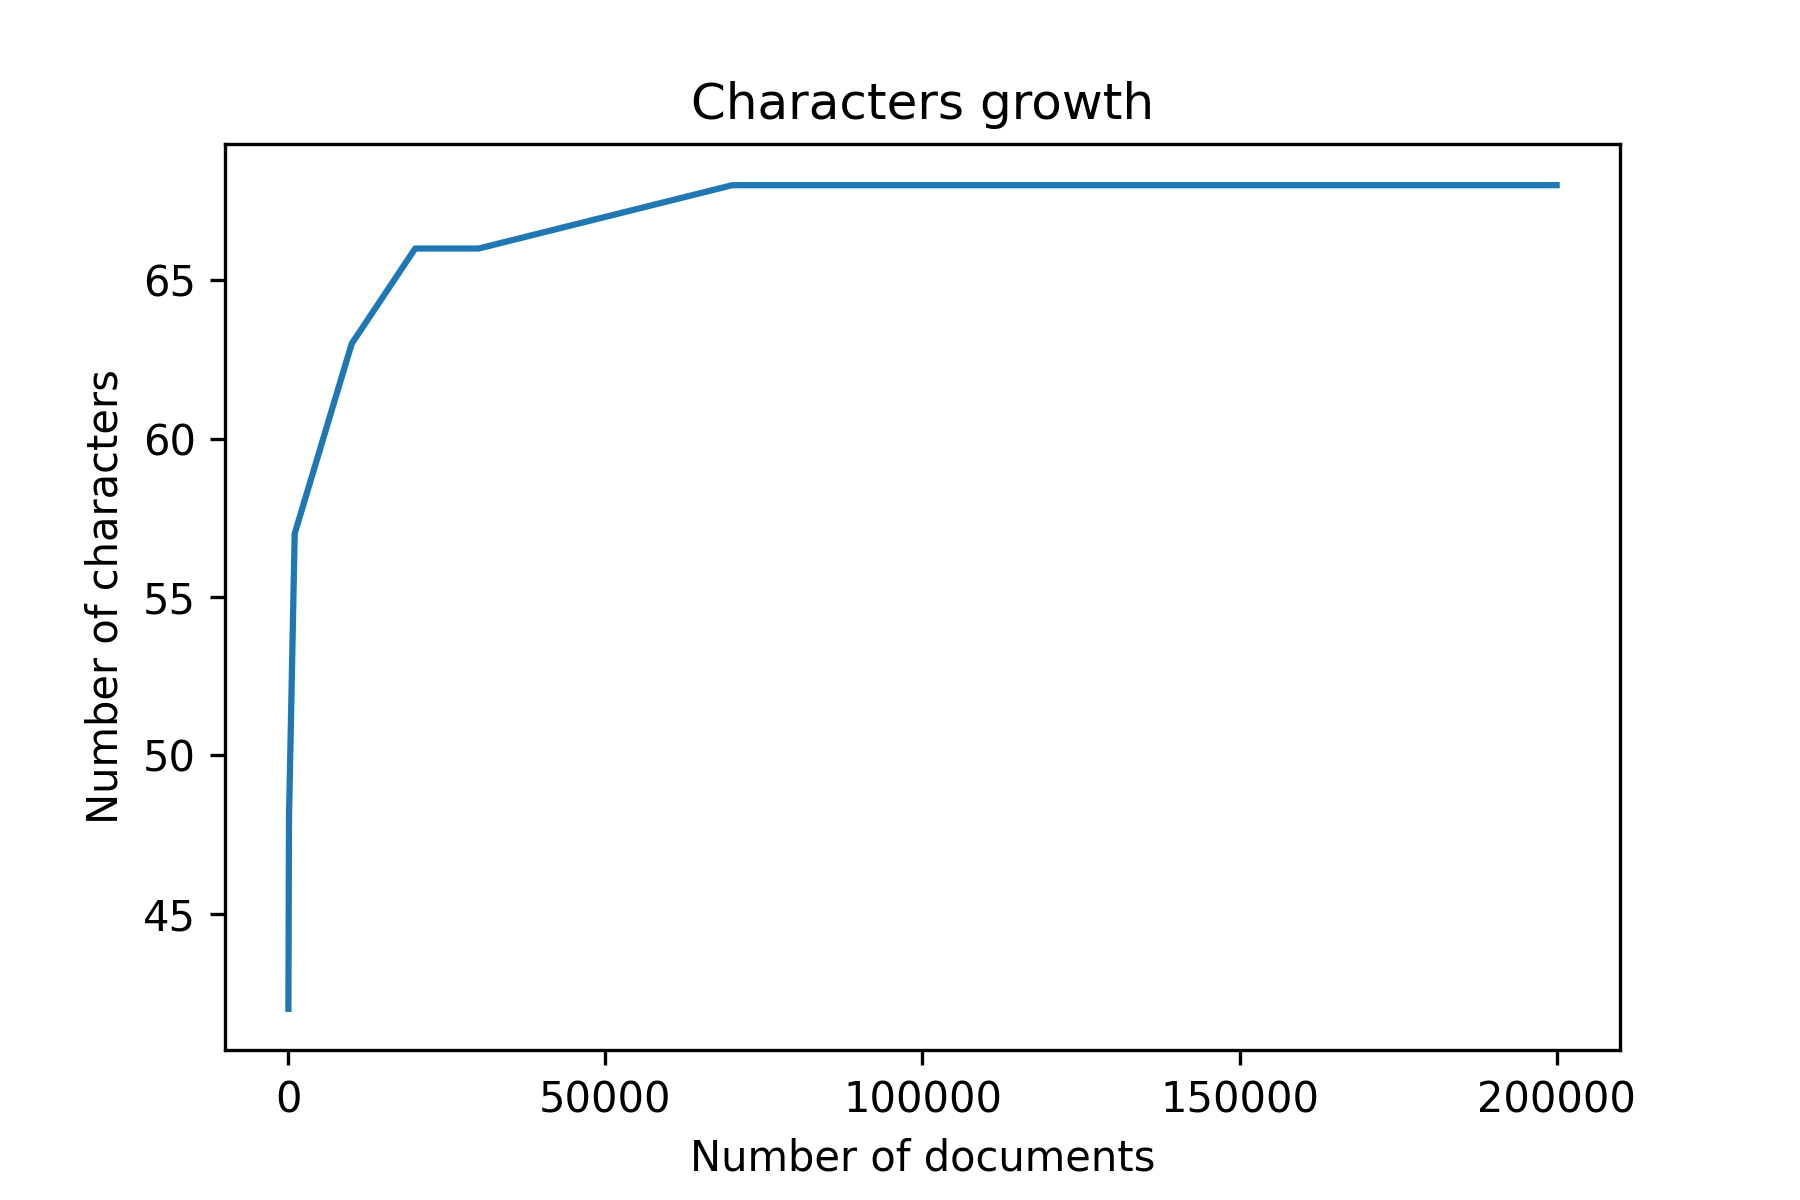
\includegraphics[width=1\textwidth]{../img/char_growth.png}
  \caption{Growth in the number of characters as the number of documents increases.} 
  \label{fig:experiments:char_growth}
\end{figure}

\begin{figure}
  \center
  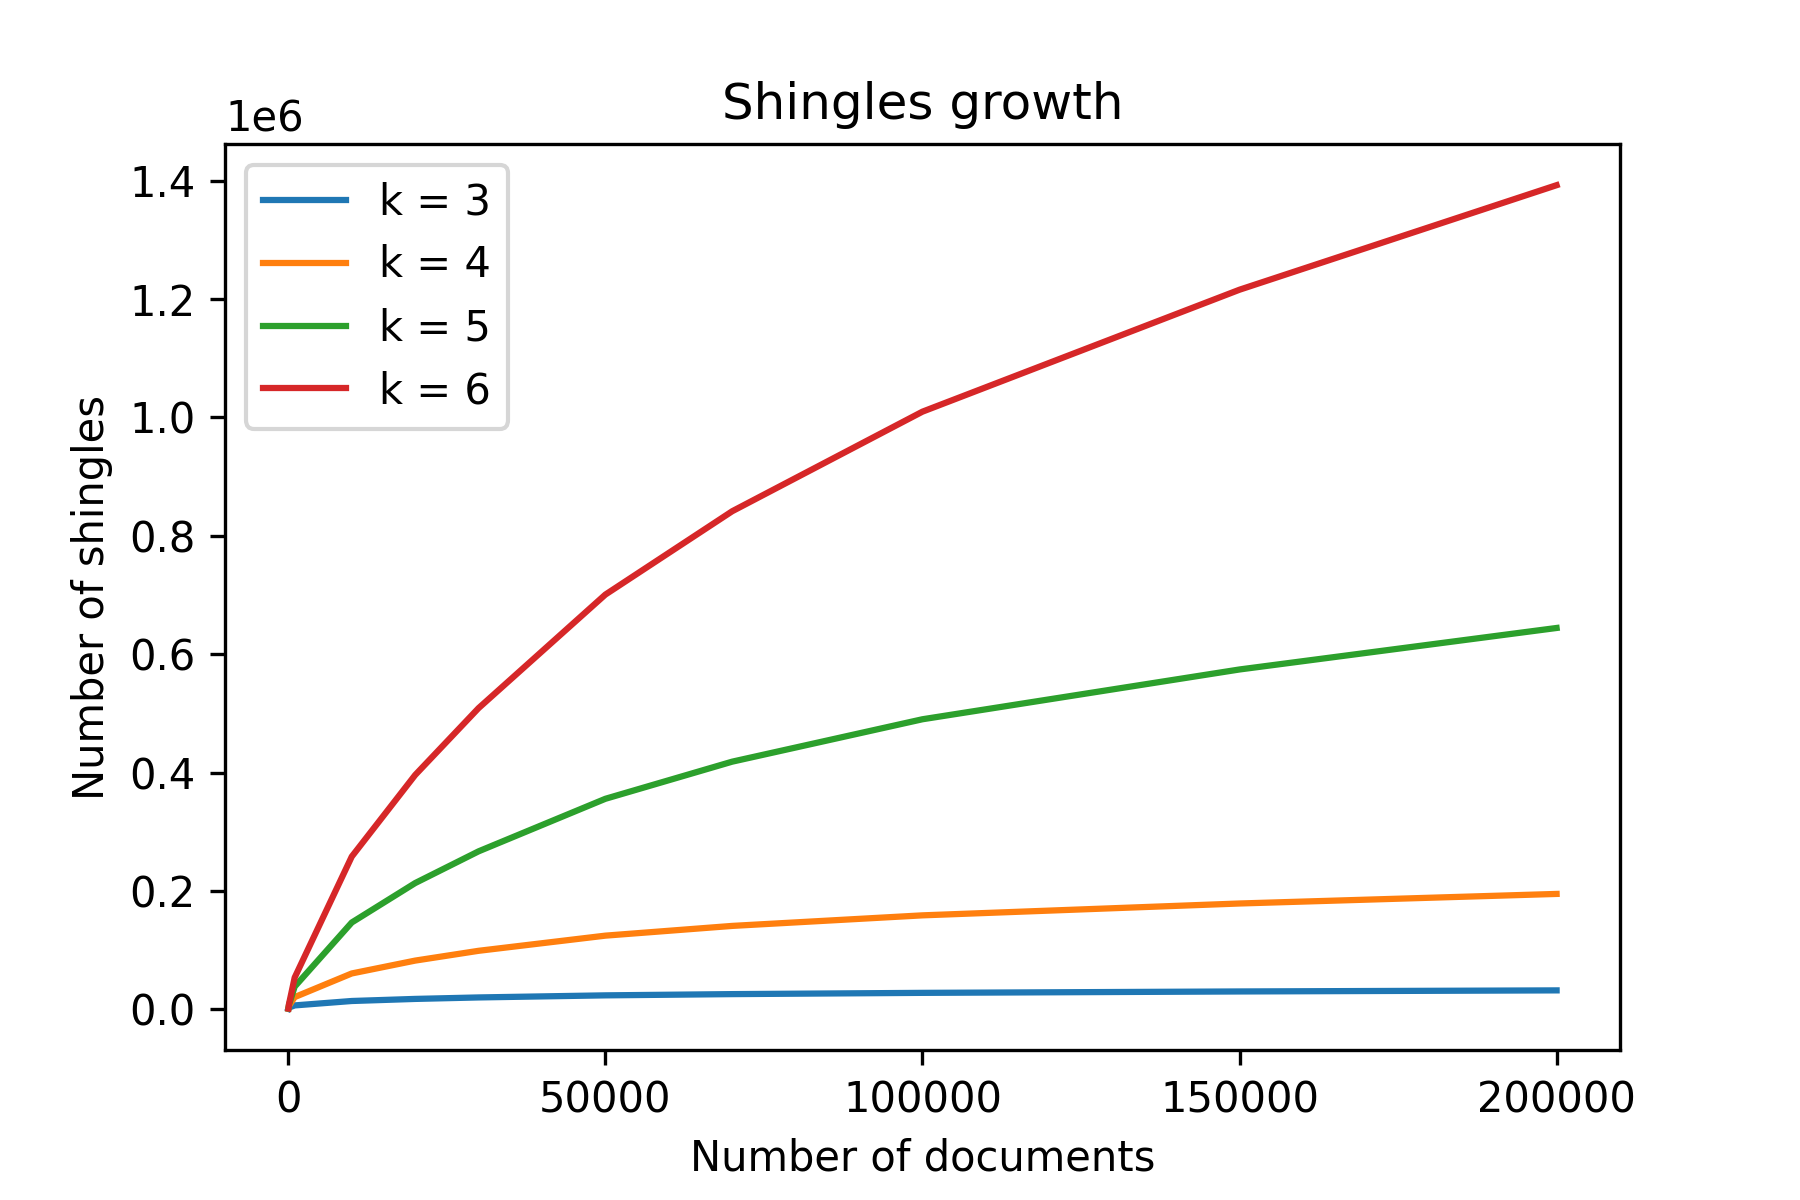
\includegraphics[width=1\textwidth]{../img/shingles_growth.png}
  \caption{Growth in the number of shingles as the number of documents increases. The growth is shown for shingles obtained with different k-grams.} 
  \label{fig:experiments:shingles_growth}
\end{figure}

In this first experiment we wanted to gauge how the number of shingles (or k-grams) and different characters within the whole corpus varied as the number of documents increased. 

In Figure~\ref{fig:experiments:char_growth} we can see how the number of characters grows as the number of documents increases. In particular, we can see how from 100.000 documents onwards the number of characters is stable at around 65 characters (68, to be precise). This is useful to get a hint on the appropriate k-gram with respect to the number of buckets of the hash function that maps k-grams to integers. For instance, given that $68^3 = 314.432$, we can infer that, if we used 3-grams, we would need a hash function with approximately 300.000 buckets.

Working with characters we can get an estimate on the number of buckets that we would need. However, it is unlikely that all the possible shingles will appear in practice. To this end, we also explored how the actual number of different shingles grows as the number of documents increases.

In Figure~\ref{fig:experiments:shingles_growth} we can see how the number of different shingles grows as the number of documents increases. It is not surprising to see that, with k-grams having a higher value of k, the number of shingles grows more steeply. We can also see, however, that this growth is approximately logarithmic in shape and stabilizes quickly for low values of k. Indeed, for k equal to 3 and 4, most of the shingles have already been found at 50.000 documents. To be precise, at 50.000 documents we have 21.580 shingles with 3-grams and 111.643 shingles with 4-grams. For 3-grams, a hash function with buckets of at least 15 bits would be enough ($2^{15} = 32.768$ buckets). For 4-grams, we would need at least 17 bits to have a fair chance at avoiding collisions ($2^{17} = 131.072$ buckets).  


\subsection{Number of Buckets}
\label{subsec:experiments:buckets}

\begin{table}
  \caption{Effects of the increase in the number of bits for the hash function that maps k-grams to integers when k is equal to 3. We highlighted in bold the best results for precision and mean absolute error (MAE).}
  \label{tab:experiments:buckets_k3}
  \centering
  \begin{tabular}{lccccc}
    \toprule
    {} &    True Positive &   False Positive &  Precision &    MAE & Time Delta \\
    Hash bits &       &      &            &        &            \\
    \midrule
    12        &  1289 &  560 &      \textbf{0.697} &  0.021 &    0:02:06 \\
    14        &   945 &  738 &      0.561 &  0.023 &    0:02:11 \\
    16        &   705 &  328 &      0.682 &  \textbf{0.018} &    0:02:28 \\
    18        &   722 &  374 &      0.659 &  0.020 &    0:03:45 \\
    19        &   767 &  500 &      0.605 &  0.019 &    0:05:27 \\
    20        &   779 &  413 &      0.654 &  0.019 &    0:08:50 \\
    22        &   713 &  457 &      0.609 &  0.020 &    0:28:55 \\
    \bottomrule
  \end{tabular}
\end{table}

In this experiment we wanted to see how increasing the number of bits of the hash function that maps k-grams to integers affected various metrics. This experiment was carried out with a fixed threshold of 0.1 and 100 hash functions for the permutations of the rows. 

The first metric we examined was precision, defined as 
\[
  \text{Precision} = \frac{\text{TP}}{\text{TP} + \text{FP}}\,,
\]
where $\text{TP}$ is the number of true positives and $\text{FP}$ is the number of false positives. TP and FP are obtained by computing the actual Jaccard similarity on the pairs of documents identified as similar by the algorithm. This was done using the characteristic matrix. Afterwards, we checked if the Jaccard similarity was indeed higher than the threshold. If not, we considered the pair a false positive.

The second metric we examined was the mean absolute error (MAE) between the similarity estimated by the algorithm and the actual Jaccard similarity. As third metric, we examined how the number of bits affected the time of execution.

In Tables~\ref{tab:experiments:buckets_k3} we can see the results for 3-grams, 4-grams and 5-grams, respectively.  

Note also that, for low value of bits, most of the time was spent reading the files.


\subsection{Threshold}
\label{subsec:experiments:threshold}

\subsection{Number of Hash Functions}
\label{subsec:experiments:hashes}

\subsection{Similarity between 100.000 Tweets}
\label{subsec:experiments:100k}



\section{Conclusions}
\label{sec:conclusions}

We could improve the algorithm by appending argument type constraints to the templates.


After feeding the documents to 

Example of similar tweets
Non-cryptographic function

and which has been found to work well  
Link a zip with checkpoints in the github
To achieve this goal
To this end

, so we removed all URLs 
beforehand. 
We also removed URLs from tweets, since that differed only in hashtags or in  placed within the messages were not filtered, since . 

might skew

each of which organized in fields providing information about the author
each of which  

foregoing

Not actually deduped.

Optimizer to find b and r
Hash in LSH
Last layer has most meaning
TFIDF? Need to traverse the whole dataset to compute, taxing operation
Two semantically different pipelines: to filter almost identical tweets, and the other.
Punctuation and non-ascii removed later, because they might help the lemmatizer
CHANGED PIPELINE (some differed for only some whitespace or for a capital letter (mint and MINT))

Problem with low threshold, ends RAM with combinations
As such, we decided to experiment with   
The algorithm 
used dictionary to store shingles 

List of documents, each with its own correlation
Check TP on final


Being confronted with the problem of finding hash functions that could map to different numbers of buckets,

filled to the brim of duplicates
no clear takeaways
more hashes more FN?

k=3 with t0.4 over 1M pairs

Strip again punctuation because some of the lemmas had punctuation symbols like \_ in them.

Retweets and Quote tweets. We assume the reader to be familiar with Twitter.

Check if quote or retweet with quote and retweet status (\url{https://developer.twitter.com/en/docs/twitter-api/v1/data-dictionary/object-model/tweet})

Filtering for followers number doesn't seem useful. Many people retweet the smae things. maybe they made mistakes.

fast spike increase in shingles at low documents

used spacy 

Cannot use spacy on dataframe, takes too much time

crash with t.02, too many pairs
with t=0.4 6346167 candidate pairs, actual 342671 

We do not drop duplicates across different files, as that would require to load in main memory millions of documents. Plenty of retweets. Plenty of very short tweets that are identical after preprocessing /lemmatization. But filtering on string length isn't suitable due to the instrinsic short nature of tweets.  
Sometimes only changed a handle or more, but removing handles might remove important parts (many quote zelensky with handle for instance).

Removing handles might be somehow questionable... Si ma poi se tanto retweettano in altri file compare comunque.

Dai, remove handle e testi più lunghi di tot...
ONLY EN language
Should have kept the retweet flag


CHECK TP ON ACTUAL OUTPUT, AFTER THRESH CHECK

Generate the combinations manually and add one at a time, to avoid ram problem?

\bibliographystyle{splncs04}
\bibliography{bibtex_entries}

\end{document}